\documentclass{article}

\usepackage{color}
\usepackage{listings}
\usepackage{fullpage}
\usepackage{graphicx}

\definecolor{gray_ulisses}{gray}{0.55}
\definecolor{castanho_ulisses}{rgb}{0.71,0.33,0.14}
\definecolor{preto_ulisses}{rgb}{0.41,0.20,0.04}
\definecolor{green_ulises}{rgb}{0.2,0.75,0}

\lstdefinelanguage{HaskellUlisses}
{
	basicstyle=\ttfamily\scriptsize,
	%backgroundcolor=\color{yellow},
	%frameshape={RYRYNYYYY}{yny}{yny}{RYRYNYYYY}, %contornos... muito nice...
	sensitive=true,
	morecomment=[l][\color{gray_ulisses}\scriptsize]{--},
	morecomment=[s][\color{gray_ulisses}\scriptsize]{\{-}{-\}},
	morestring=[b]",
	stringstyle=\color{red},
	showstringspaces=false,
	numbers=none,
	firstnumber=\thelstnumber,
	numberstyle=\tiny,
	numberblanklines=true,
	showspaces=false,
	showtabs=false,
	xleftmargin=15pt,
	xrightmargin=-20pt,
	emph=
	{[1]
		FilePath,IOError,abs,acos,acosh,all,and,any,appendFile,approxRational,asTypeOf,asin,
		asinh,atan,atan2,atanh,basicIORun,break,catch,ceiling,chr,compare,concat,concatMap,
		const,cos,cosh,curry,cycle,decodeFloat,denominator,digitToInt,div,divMod,drop,
		dropWhile,either,elem,encodeFloat,enumFrom,enumFromThen,enumFromThenTo,enumFromTo,
		error,even,exp,exponent,fail,filter,flip,floatDigits,floatRadix,floatRange,floor,
		fmap,foldl,foldl1,foldr,foldr1,fromDouble,fromEnum,fromInt,fromInteger,fromIntegral,
		fromRational,fst,gcd,getChar,getContents,getLine,head,id,inRange,index,init,intToDigit,
		interact,ioError,isAlpha,isAlphaNum,isAscii,isControl,isDenormalized,isDigit,isHexDigit,
		isIEEE,isInfinite,isLower,isNaN,isNegativeZero,isOctDigit,isPrint,isSpace,isUpper,iterate,
		last,lcm,length,lex,lexDigits,lexLitChar,lines,log,logBase,lookup,map,mapM,mapM_,max,
		maxBound,maximum,maybe,min,minBound,minimum,mod,negate,not,notElem,null,numerator,odd,
		or,ord,otherwise,pi,pred,primExitWith,print,product,properFraction,putChar,putStr,putStrLn,quot,
		quotRem,range,rangeSize,read,readDec,readFile,readFloat,readHex,readIO,readInt,readList,readLitChar,
		readLn,readOct,readParen,readSigned,reads,readsPrec,realToFrac,recip,rem,repeat,replicate,return,
		reverse,round,scaleFloat,scanl,scanl1,scanr,scanr1,seq,sequence,sequence_,show,showChar,showInt,
		showList,showLitChar,showParen,showSigned,showString,shows,showsPrec,significand,signum,sin,
		sinh,snd,span,splitAt,sqrt,subtract,succ,sum,tail,take,takeWhile,tan,tanh,threadToIOResult,toEnum,
		toInt,toInteger,toLower,toRational,toUpper,truncate,uncurry,undefined,unlines,until,unwords,unzip,
		unzip3,userError,words,writeFile,zip,zip3,zipWith,zipWith3,Impl,Equiv,Prop,Neg,Cnj,Dsj
	},
	emphstyle={[1]\color{blue}},
	emph=
	{[2]
		Bool,Char,Double,Either,Float,IO,Integer,Int,Maybe,Ordering,Rational,Ratio,ReadS,ShowS,String,NoTriangle,Equilateral,Rectangular,Isosceles,Other,Shape
	},
	emphstyle={[2]\color{castanho_ulisses}},
	emph=
	{[3]
		case,class,data,deriving,do,else,if,import,in,infixl,infixr,instance,let,
		module,of,primitive,then,type,where
	},
	emphstyle={[3]\color{preto_ulisses}\textbf},
	emph=
	{[4]
		quot,rem,div,mod,elem,notElem,seq
	},
	emphstyle={[4]\color{castanho_ulisses}\textbf},
	emph=
	{[5]
		EQ,False,GT,Just,LT,Left,Nothing,Right,True,Show,Eq,Ord,Num
	},
	emphstyle={[5]\color{preto_ulisses}\textbf}
}

\lstnewenvironment{code}
{\lstset{language=HaskellUlisses}}
{\smallskip}


\begin{document}
\setlength{\parindent}{0cm}

\title{Software Testing Assignment 3}
\author{Cindy Berghuizen, Omar Pakker , Chiel Peter, Maria Gouseti}
\date{22 September , 2013}
\maketitle
\section*{Exercise 5}

\subsection*{Properties}
The testable properties we defined and used in our version of $isPermutation$
are (see figure~\ref{fig:isPermutation}):
\begin{itemize}
 \item an empty list is a permutation of an empty list
 \item both lists have the same length (the first list is empty and the second one still has elements)
 \item A list $L'$ is a permutation of a list $L$ if every appearance of an
element that exists in list $L$ also exists in $L'$ and $L'$ does not have other elements.
\end{itemize}

\subsection*{Testing}
In order to test $isPermutation$ we are going to use $permutations$ a function from Haskell
Data.List. This function gets a list as an argument and returns a
list we all its permutations, including the initial list as well. Consequently
we check if the the second argument of $isPermutation$ is an element of the list
created by $permutations$ with argument the first list. If both functions have
the same value $isPermutation$ is correct. We also created
$testPermutationsTotal$ which presents if all the test were successful (see figure~\ref{fig:testPermutationsTotal}).

\begin{code}
--Exercise 5
testPermutation :: IO Bool
testPermutation = do
			     p1 <- genIntList
			     p2 <- genIntList
			     return ((isPermutation p1 p2) == (elem p2 (permutations p1)))

testPermutations :: Int -> IO [Bool]
testPermutations 0 = return []
testPermutations c = do
			     p <- testPermutation
			     ps <- testPermutations (c-1)
			     return (p:ps)

testPermutationsTotal :: Int -> IO String
testPermutationsTotal c = do
			     ps <- testPermutations c
			     return ("All Checks Valid: " ++ (show (all (\x -> x) ps)))
\end{code}

\begin{figure}[ht]
\begin{minipage}[b]{0.5\linewidth}
\centering
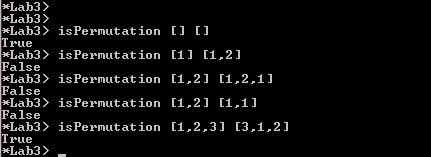
\includegraphics[width=\textwidth]{isPermutation_manual.jpg}
\caption{Manual execution of $isPermutation$ testing the properties mentioned above.}
\label{fig:isPermutation}
\end{minipage}
\hspace{0.5cm}
\begin{minipage}[b]{0.5\linewidth}
\centering
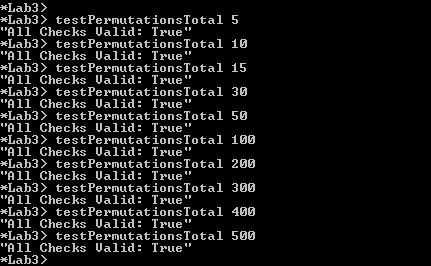
\includegraphics[width=\textwidth]{testPermutationsTotal.jpg}
\caption{$testPermutationsTotal$}
\label{fig:testPermutationsTotal}
\end{minipage}
\end{figure}


\section*{Exercise 6}
When we started testing our CNF converter using our random formula generator we
noticed that we have missed the case of an empty disjunction as a result in
this case the function did not work properly. So we added a line to catch this
case in order to test the function. The fixed code of our CNF converter:

\begin{code}
-- Precondition: Form is arrowfree and in negative normal form
-- Postcondition: Form is in conjunctive normal form
cnf :: Form -> Form
cnf (Prop x)		= Prop x
cnf (Neg (Prop x))	= Neg (Prop x)
cnf (Cnj f)		= Cnj (map cnf f)
cnf (Dsj []) = Dsj [] --Added 2013-09-16; previously missed
cnf (Dsj [f, g])	= dist (cnf f) (cnf g)
cnf (Dsj (f:fs))	= dist (cnf f) (cnf (Dsj fs))

-- Precondition: Forms are in conjunctive normal form
-- Postcondition: Form is the the conjunctive normal form of (form1 v form2)
dist :: Form -> Form -> Form
dist (Cnj fs) g 	= Cnj (map (dist g) fs)
dist f (Cnj gs)		= Cnj (map (dist f) gs)
dist f g 		= Dsj [f,g]

\end{code}

To test the CNF converter we used two functions that approach it differently.
The first one is $equiv$ from assignment 2. With this function we can test that
the original form and its CNF version are equivalent ($testCNF$). Then we
changed the parser of predicate logic to accept only forms in CNF ($parseCNF$ as shown in figure~\ref{fig:parseCNF}).
If the result of our CNF converter passes both tests then the CNF converter is
correct. The function $showCNFResults$ returns the score of the correct conversions (see figure~\ref{fig:showCNFResults}).

\begin{figure}[ht]
\begin{minipage}[b]{0.5\linewidth}
\centering
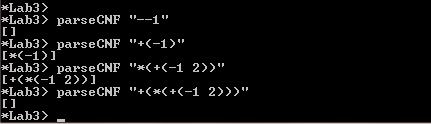
\includegraphics[width=\textwidth]{parseCNF.jpg}
\caption{$parseCNF$ returns $[]$ when its argument is not in CNF.}
\label{fig:parseCNF}
\end{minipage}
\hspace{0.5cm}
\begin{minipage}[b]{0.5\linewidth}
\centering
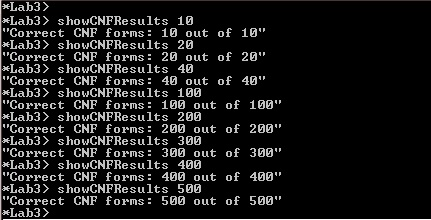
\includegraphics[width=\textwidth]{CNFtest.jpg}
\caption{$showCNFResults$}
\label{fig:showCNFResults}
\end{minipage}
\end{figure}

\begin{code}
showCNFResults n = do
		      r <- (testCNFs n)
		      return ("Correct CNF forms: "++(show (length (filter ((==)
				True) r)))++" out of "++(show (length r)))

testCNFs n = do
		      g <- (getRandomFs n)
		      return (map ( \x -> testCNF x) g)
 
testCNF f = (equiv f g) && ((parseCNF (formToString g))/=[]) where g = (cnf (nnf f))
 
formToString :: Form -> String
formToString form = show form

parseCNFForm :: Int->(Parser Token Form) 
parseCNFForm i (TokenInt x: tokens) = [(Prop x,tokens)]
parseCNFForm i (TokenNeg: TokenInt x : tokens) = [ (Week2.Neg (Prop x), tokens)]
parseCNFForm i (TokenCnj : TokenOP : tokens) | i==0 = [ (Dsj fs, rest) | (fs,rest) <- parseCNFForms i tokens ]
					     | otherwise = []
parseCNFForm i (TokenDsj : TokenOP : tokens) = [ (Cnj fs, rest) | (fs,rest) <- parseCNFForms (i+1) tokens ]
parseCNFForm i tokens = []

parseCNFForms :: Int-> (Parser Token [Form]) 
parseCNFForms i (TokenCP : tokens) = succeed [] tokens
parseCNFForms i tokens = [(f:fs, rest) | (f,ys) <- parseCNFForm i tokens, (fs,rest) <- parseCNFForms i ys ]

parseCNF :: String -> [Form]
parseCNF s = [ f | (f,_) <- parseCNFForm 0 (lexer s) ]
\end{code}



\end{document}